\chapter{Resultados} \label{cap:resultados}
\vspace{-2cm}

Após as correções da simulação explicadas no Capítulo \ref{cap:simulacao} Sessão \ref{sec:bugs}, encontramos a qualidade da água $70\%$ pior do que uma água pura. Os histogramas de energia podem ser vistos nas Figuras \ref{fig:a5} e \ref{fig:b4}. A curva de transformação está representada na Figura \ref{fig:transf}.


\begin{figure}[H]
	\centering
	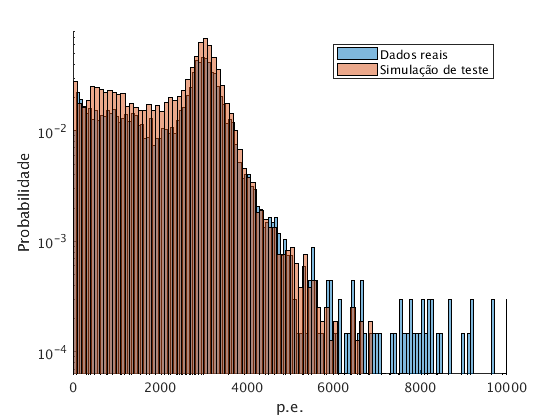
\includegraphics[width=10cm]{textuais/simulacao/figuras/hist_evt4.png}
	\caption{Histograma da energia por eventos com a qualidade da água 70\% pior que a original}
	\label{fig:a5}
\end{figure}

\begin{figure}[H]
	\centering
	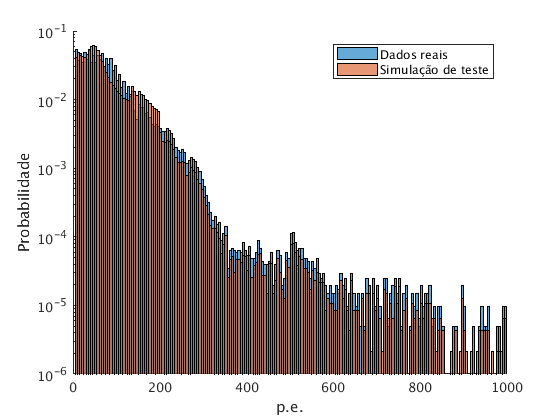
\includegraphics[width=10cm]{textuais/simulacao/figuras/hist_pmt4.png}
	\caption{Histograma da energia por PMT com a qualidade da água 70\% pior que a original}
	\label{fig:b4}
\end{figure}

\begin{figure}[H]
	\centering
	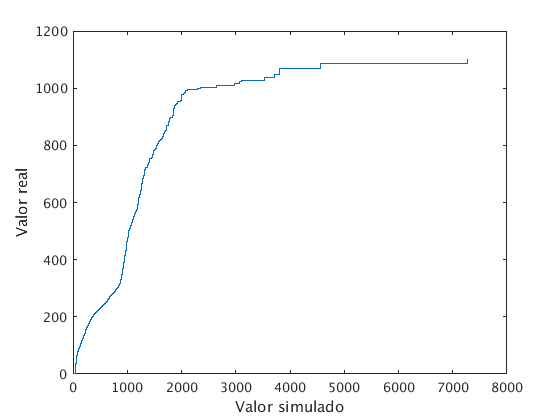
\includegraphics[width=10cm]{textuais/simulacao/figuras/cdfe.png}
	\caption{Transformação de CDFe dos valores simulados para valores reais }
	\label{fig:transf}
\end{figure}


Pôde ser visto uma distorção no histograma de energia por PMT (Figura \ref{fig:b4}) após o método da CDFe, este erro pode ser atribuído à transição de transformação e os valores originais da simulação. Este problema modifica a distribuição (probabilidade) das energias porém mantém o formato da transformação.